\chapter{Trigger efficiency measurements for the search for invisibly decaying Higgs bosons in Run 2 data}
\label{chap:run2}

%??CHECK PLOT AXIS LABEL SIZES AND THAT LEGEND TERMS ARE STANDARD OR IN TEXT
%??succinct summary of run 2 trigger efficiencies
The trigger efficiency measurements performed for the Run 1 \ac{VBF} parked data analysis were repeated for the trigger used for the Run 2 2015 data analysis.
%??1D efficiencies, describe 3D efficiencies say similar results to run 1

\begin{figure}
  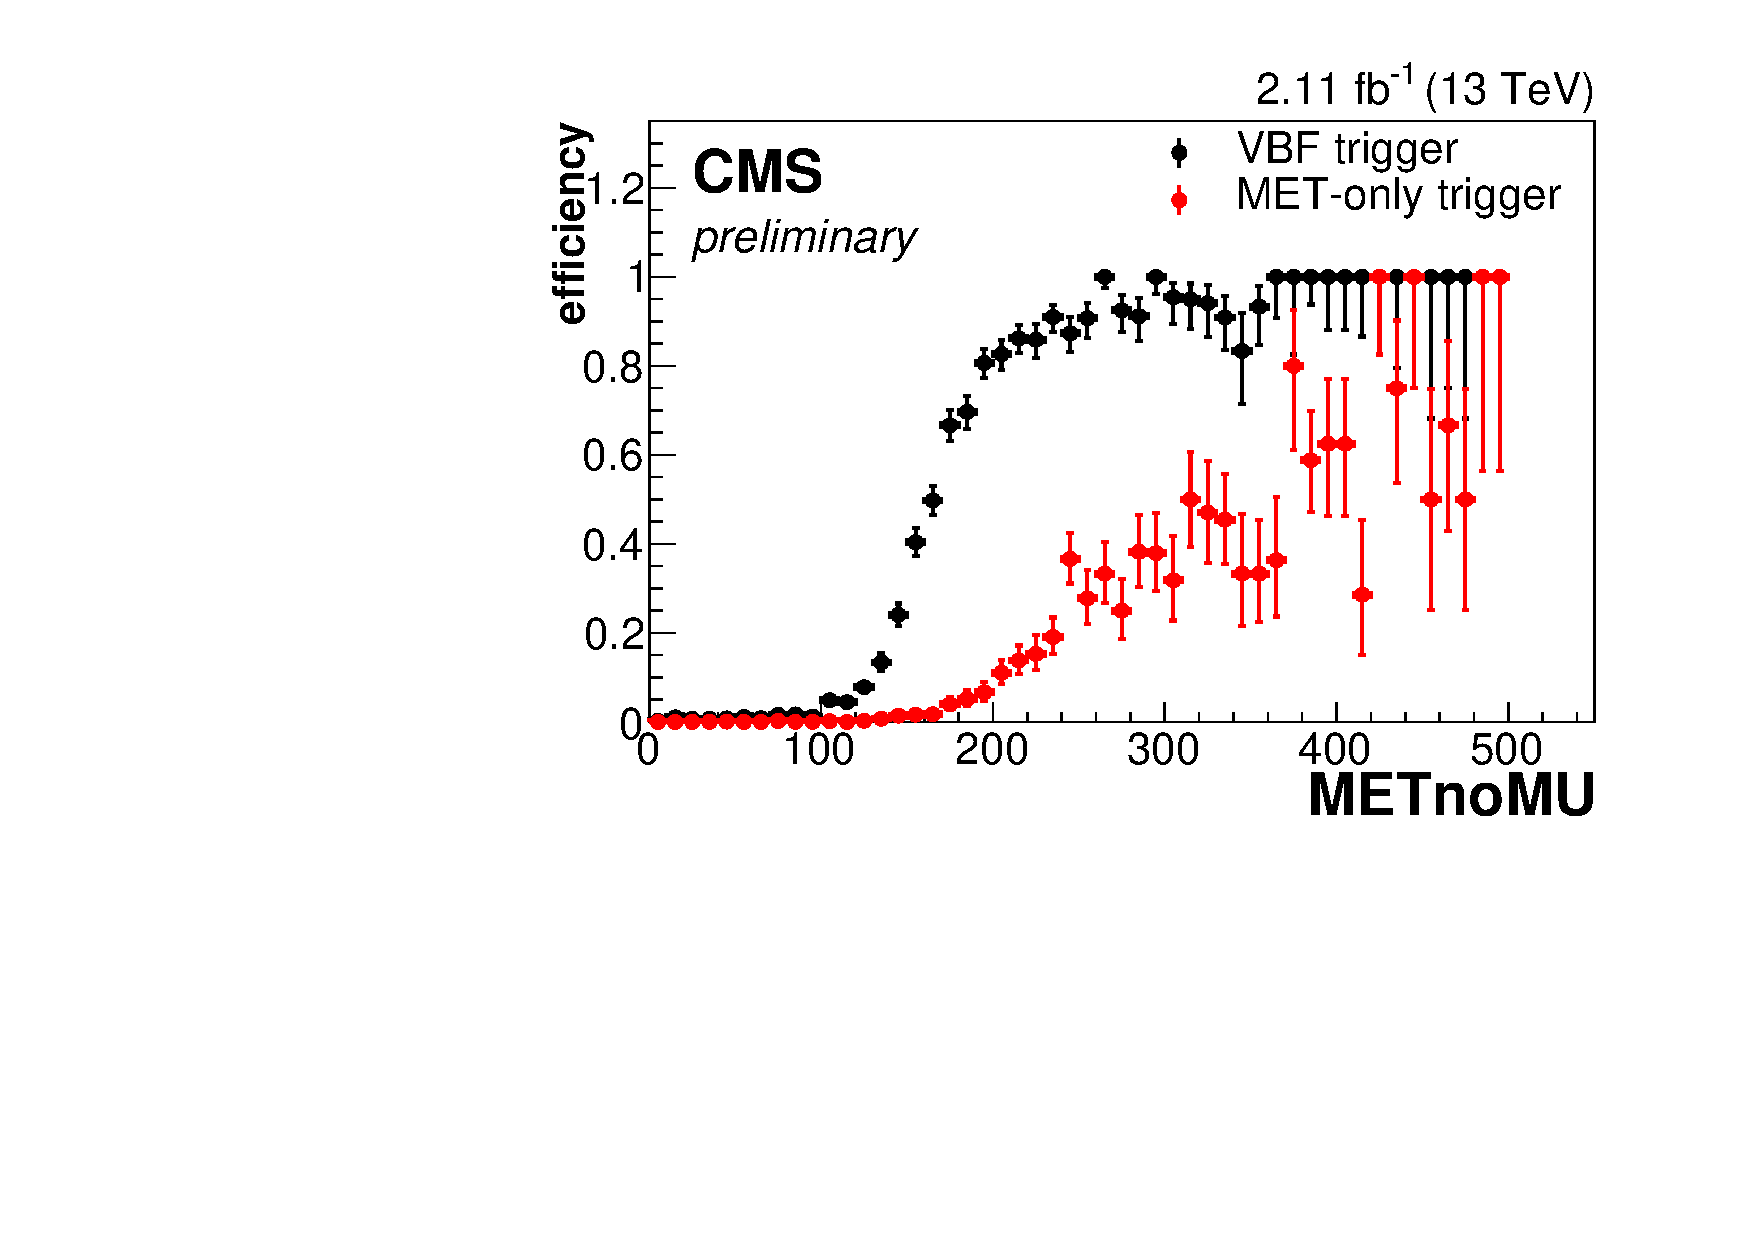
\includegraphics[width=\largefigwidth]{plots/run2/output_2015Dtrigeff_131115json_sigtrig_031215/nunu_metnomuons.pdf}
  \caption{Efficiency of VBF Higgs to invisible trigger and MET only trigger in single muon data as a function of MET ignoring muons (METnoMU). The denominator of the efficiency is the number of events passing a single muon trigger which have two jets with \pt$> 80$ \GeV, $M_{jj}>600$ \GeV and \detajj$> 3.6$ \GeV.}
  \label{fig:run2meteff}
\end{figure}

\begin{figure}
  \subfloat[]{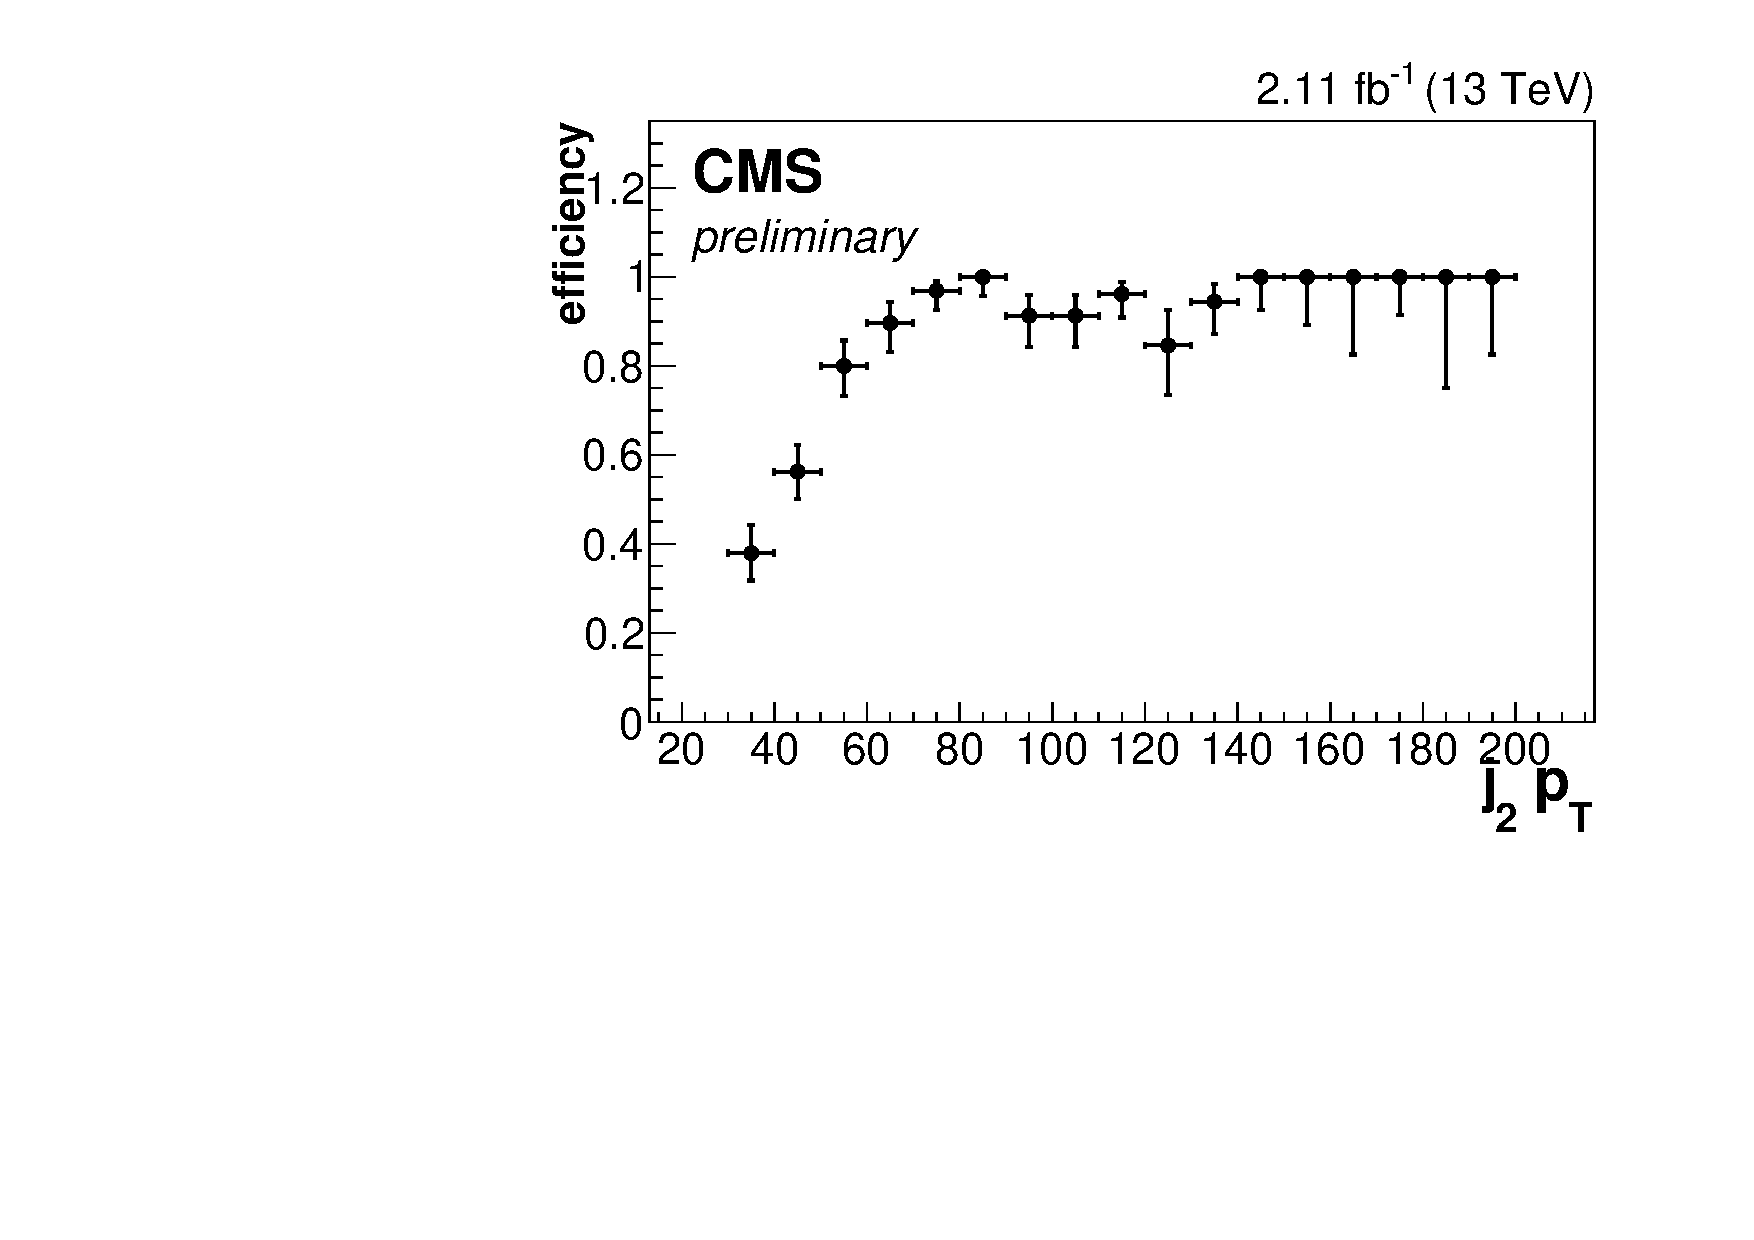
\includegraphics[width=.65\largefigwidth]{plots/run2/output_2015Dtrigeff_131115json_sigtrig_031215/nunu_jet2_pt.pdf}}
  \subfloat[]{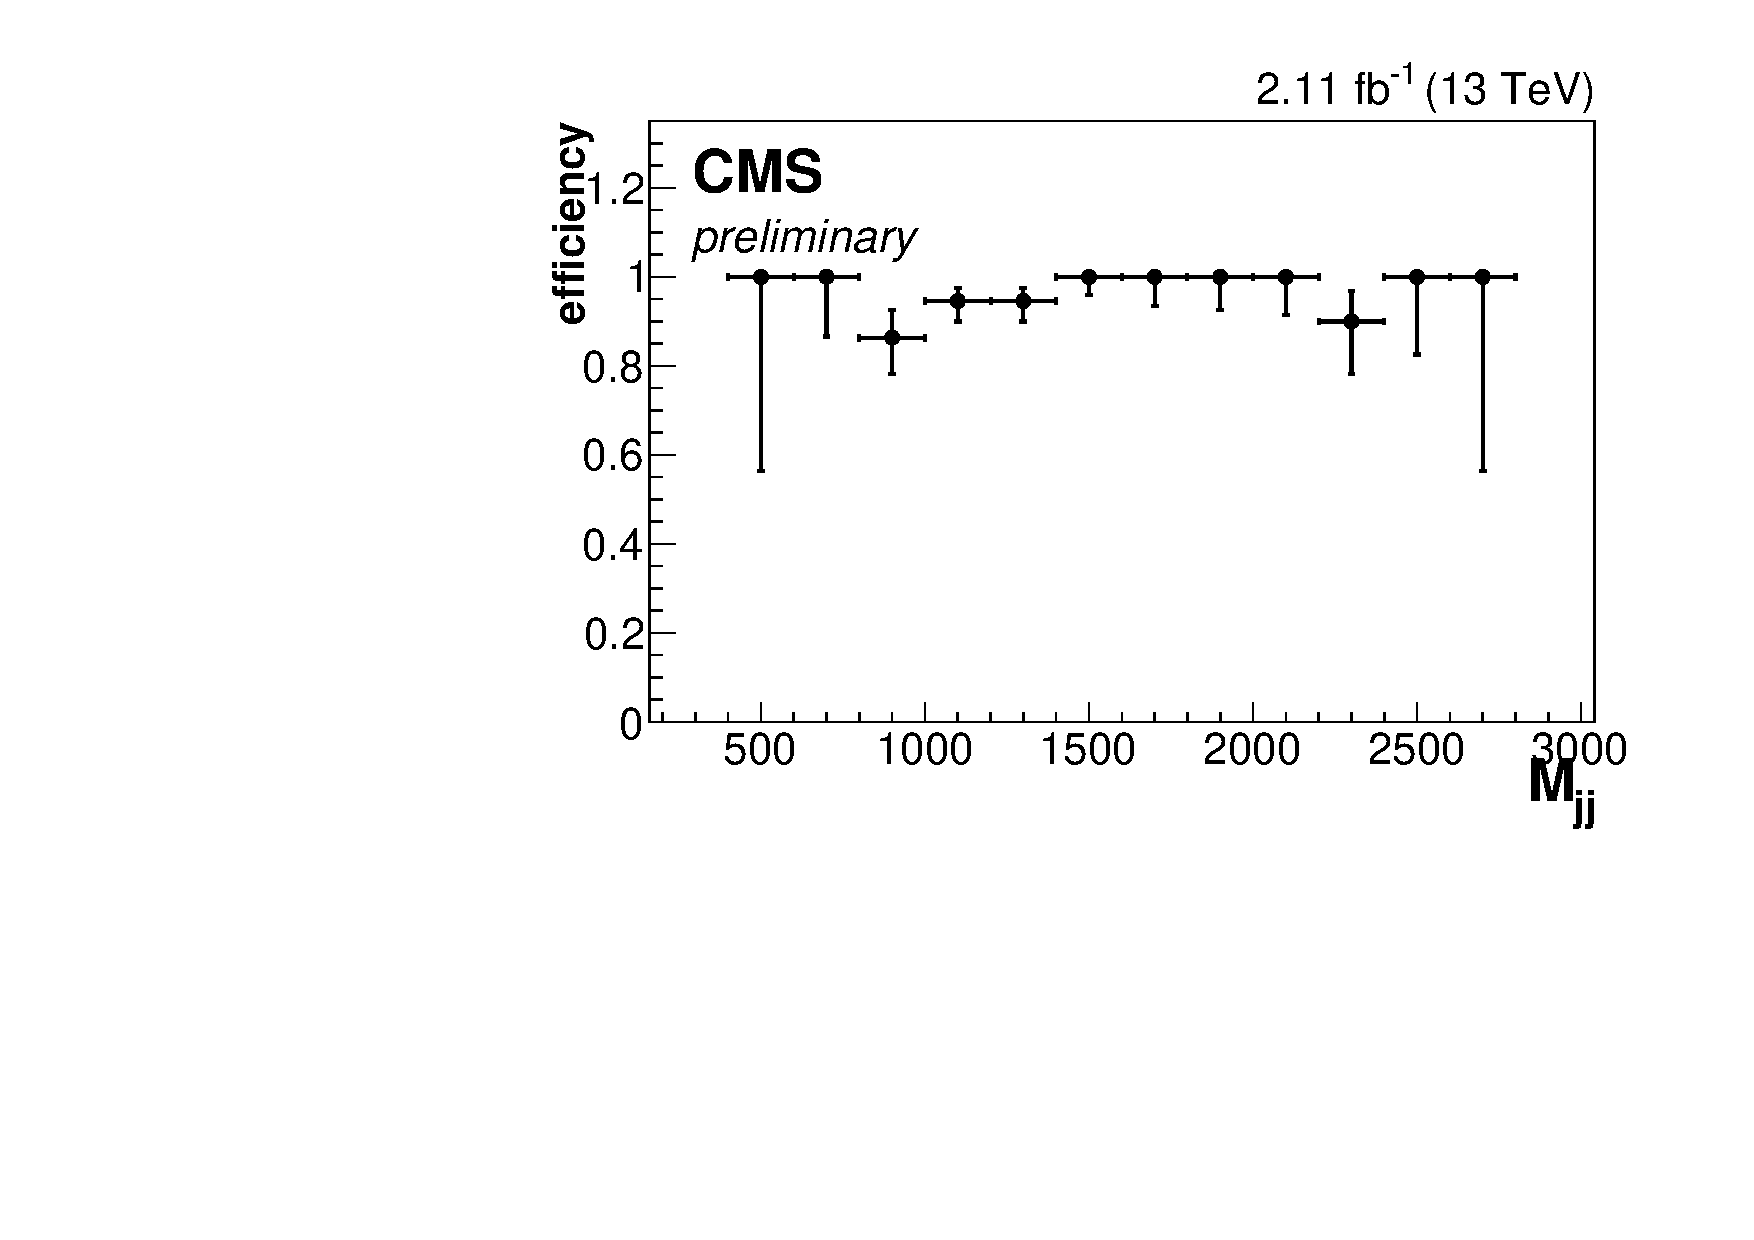
\includegraphics[width=.65\largefigwidth]{plots/run2/output_2015Dtrigeff_131115json_sigtrig_031215/nunu_dijet_M.pdf}}

  \subfloat[]{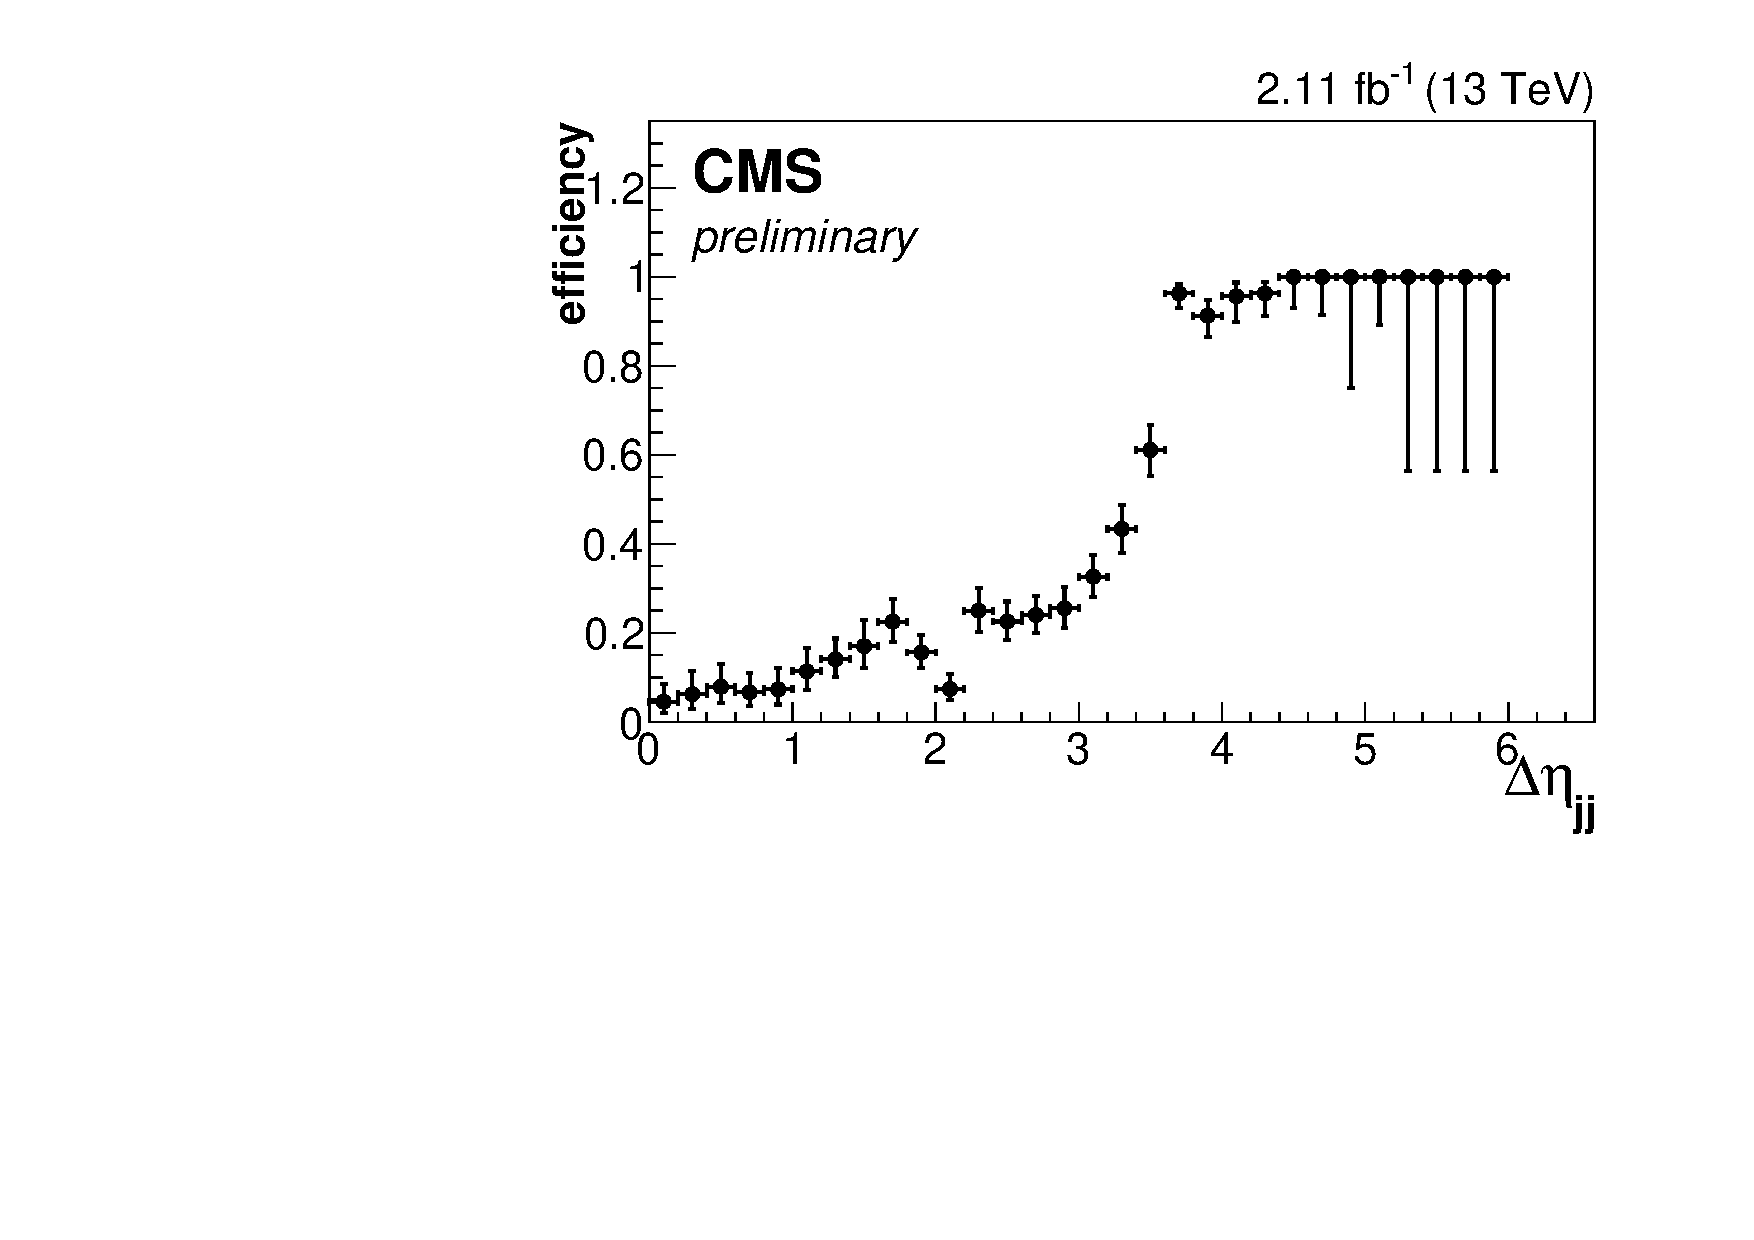
\includegraphics[width=.65\largefigwidth]{plots/run2/output_2015Dtrigeff_131115json_sigtrig_031215/nunu_dijet_deta.pdf}}
  \caption{Efficiency of VBF Higgs to invisible trigger in single muon data as a function of sub-leading jet \pt (a), \Mjj (b) and \detajj (c). The denominator of the efficiency is the number of events passing a single muon trigger which have two jets with \pt$> 80$ \GeV, $M_{jj}>600$ \GeV and \detajj$> 3.6$ \GeV.}
  \label{fig:run2othereffs}
\end{figure}

